\documentclass[letterpaper,8pt,landscape]{article}

\usepackage{multicol}
\usepackage{amsmath}
\usepackage{amsfonts}
\usepackage{amssymb}
\usepackage[margin=0.75in]{geometry}
\usepackage{graphicx}

%\usepackage[dvips]{hyperref}


\newcommand{\di}{\displaystyle}
\newcommand{\R}{\mathbb{R}}
\newcommand{\aaa}{\mathbf{a}}
\newcommand{\bbb}{\mathbf{b}}
\newcommand{\ccc}{\mathbf{c}}
\newcommand{\dotp}{\boldsymbol{\cdot}}
\newcommand{\abs}[1]{\lvert #1\rvert}
\newcommand{\len}[1]{\lVert #1\rVert}
\newcommand{\ivec}{\,\boldsymbol{\hat{\imath}}}
\newcommand{\jvec}{\,\boldsymbol{\hat{\jmath}}}
\newcommand{\kvec}{\,\boldsymbol{\hat{k}}}
\newcommand{\bvm}{\begin{vmatrix}}
\newcommand{\evm}{\end{vmatrix}}

\title{Potentially useful facts and definitions}
\author{}

\begin{document}
\begin{center}
{\bf List of potentially useful facts and definitions} (you may remove this page)
\end{center}
\begin{multicols}{2}
\subsubsection*{Complex numbers}
\begin{itemize}
 \item Addition: $(a+ib)+(c+id) = (a+c)+i(b+d)$
 \item Multiplication: $(a+ib)(c+id) = (ac-db)+i(ad+bc)$
 \item Conjugate: $\overline{a+ib} = a-ib$
 \item Modulus: $\abs{a+ib} = \sqrt{a^2+b^2}$. (Note $\abs{z}^2 = z\overline{z}$.)
 \item Reciprocals (for division): $\dfrac{1}{z} = \dfrac{\overline{z}}{z\overline{z}} = \dfrac{1}{\abs{z}^2}\overline{z}$.
 \item Euler's formula: $\cos\theta+i\sin\theta = e^{i\theta}$. (Also written as $\operatorname{cis}\theta$.)
 \item Polar form: $a+ib = re^{i\theta}$, where $r=\abs{a+ib}$ and $\tan\theta = \dfrac{b}{a}$.
\end{itemize}
\subsubsection*{Vectors}
\begin{itemize}
 \item Vector from $A=(a_1,a_2,a_3)$ to $B=(b_1,b_2,b_3)$: 
 \[
 \vec{v} = \overrightarrow{AB} = \langle b_1-a_1, b_2-a_2, b_3-a_3\rangle.
 \]
 \item Position vector for $P=(x,y,z)$: $\vec{p} = \overrightarrow{OP} = \langle x,y,z\rangle$.
 \item Vector addition: 
\[
\vec{v}+\vec{w} = \langle v_1,v_2,v_3\rangle + \langle w_1,w_2,w_3\rangle = \langle v_1+w_1,v_2+w_2,v_3+w_3\rangle. 
\]
 \item Scalar multiplication: $c\vec{v} = c\langle v_1,v_2,v_3\rangle = \langle cv_1,cv_2,cv_3\rangle$.
 \item Magnitude (length): $\len{\vec{v}} = \len{\langle v_1,v_2,v_3\rangle} = \sqrt{v_1^2+v_2^2+v_3^2}$.
 \item Dot product: $\langle v_1,v_2,v_3\rangle\dotp \langle w_1,w_2,w_3\rangle = v_1w_1+v_2w_2+v_3w_3$.
 \item Cross product: using the notation $\bvm a&b\\c&d\evm = ad-bc$,
\[\langle v_1,v_2,v_3\rangle\times \langle w_1,w_2,w_3\rangle = \bvm v_2&v_3\\w_2&w_3\evm \hat{\imath} - \bvm v_1&v_3\\w_1&w_3\evm\hat{\jmath} + \bvm v_1&v_2\\w_1&w_2\evm\hat{k}.
\]

 \item Projection: $\operatorname{proj}_{\vec{u}}\vec{v} = \left(\dfrac{\vec{u}\dotp\vec{v}}{\vec{u}\dotp\vec{u}}\right)\vec{u}$.
\end{itemize}
\subsubsection*{Lines and Planes}
\begin{itemize}
 \item Line through $P_0 = (x_0,y_0,z_0)$ in the direction of $\vec{v} = \langle a,b,c\rangle$:
\[
 \langle x,y,z\rangle = \langle x_0,y_0,z_0\rangle + t\langle a,b,c\rangle = \vec{p}_0+t\vec{v}.
\]
 \item Plane through $P_0 = (x_0,y_0,z_0)$ with normal vector $\vec{n} = \langle A,B,C\rangle$: $\vec{n}\dotp (\vec{p}-\vec{p}_0) = A(x-x_0)+B(y-y_0)+C(z-z_0) = 0$.
\end{itemize}
\subsubsection*{The Unit Circle}
\begin{center}
 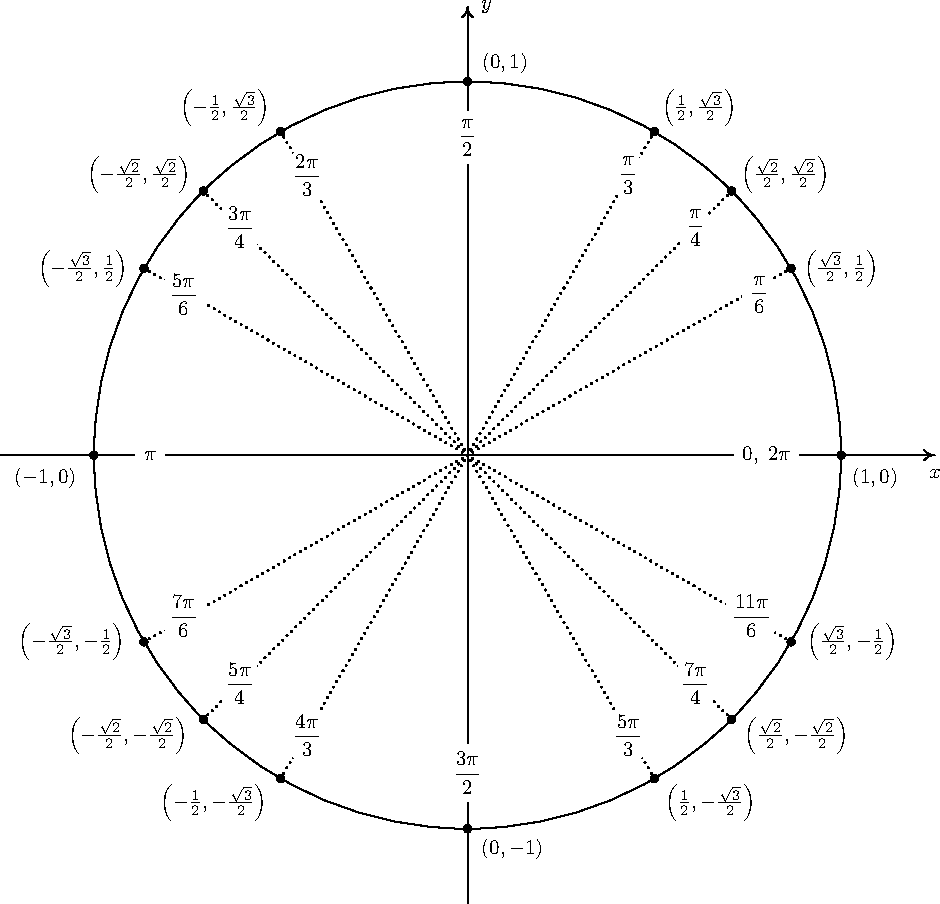
\includegraphics[width=\columnwidth]{UnitCircle}
\end{center}

\end{multicols}

\end{document}
